%%%%%%%%%%%%%%%%%%%%%%%%%%%%%%%%%%%%%%%%%
% Journal Article
% Distributed Parallel System
% Practical 1: Speeding up performance with openmp
%
% Gahan M. Saraiya
% 18MCEC10
%
%%%%%%%%%%%%%%%%%%%%%%%%%%%%%%%%%%%%%%%%%
%----------------------------------------------------------------------------------------
%       PACKAGES AND OTHER DOCUMENT CONFIGURATIONS
%----------------------------------------------------------------------------------------
\documentclass[paper=letter, fontsize=12pt]{article}
\usepackage[english]{babel} % English language/hyphenation
\usepackage{amsmath,amsfonts,amsthm} % Math packages
\usepackage[utf8]{inputenc}
\usepackage{xcolor}
\usepackage{float}
\usepackage{lipsum} % Package to generate dummy text throughout this template
\usepackage{blindtext}
\usepackage{graphicx} 
\usepackage{caption}
\usepackage{subcaption}
\usepackage[sc]{mathpazo} % Use the Palatino font
\usepackage[T1]{fontenc} % Use 8-bit encoding that has 256 glyphs
\usepackage{bbding}  % to use custom itemize font
\linespread{1.05} % Line spacing - Palatino needs more space between lines
\usepackage{microtype} % Slightly tweak font spacing for aesthetics
\usepackage[hmarginratio=1:1,top=32mm,columnsep=20pt]{geometry} % Document margins
\usepackage{multicol} % Used for the two-column layout of the document
%\usepackage[hang, small,labelfont=bf,up,textfont=it,up]{caption} % Custom captions under/above floats in tables or figures
\usepackage{booktabs} % Horizontal rules in tables
\usepackage{float} % Required for tables and figures in the multi-column environment - they need to be placed in specific locations with the [H] (e.g. \begin{table}[H])
\usepackage{hyperref} % For hyperlinks in the PDF
\usepackage{lettrine} % The lettrine is the first enlarged letter at the beginning of the text
\usepackage{paralist} % Used for the compactitem environment which makes bullet points with less space between them
\usepackage{abstract} % Allows abstract customization
\renewcommand{\abstractnamefont}{\normalfont\bfseries} % Set the "Abstract" text to bold
\renewcommand{\abstracttextfont}{\normalfont\small\itshape} % Set the abstract itself to small italic text
\usepackage{titlesec} % Allows customization of titles

%Importing csv as table
\usepackage{csvsimple}

\usepackage{makecell}
\usepackage{longtable}
\renewcommand\thesection{\Roman{section}} % Roman numerals for the sections
\renewcommand\thesubsection{\Roman{subsection}} % Roman numerals for subsections
%----------------------------------------------------------------------------------------
%       DATE FORMAT
%----------------------------------------------------------------------------------------
\usepackage{datetime}
\newdateformat{monthyeardate}{\monthname[\THEMONTH], \THEYEAR}
%----------------------------------------------------------------------------------------

\titleformat{\section}[block]{\large\scshape\centering}{\thesection.}{1em}{} % Change the look of the section titles
\titleformat{\subsection}[block]{\large}{\thesubsection.}{1em}{} % Change the look of the section titles
\newcommand{\horrule}[1]{\rule{\linewidth}{#1}} % Create horizontal rule command with 1 argument of height
\usepackage{fancyhdr} % Headers and footers
\pagestyle{fancy} % All pages have headers and footers
\fancyhead{} % Blank out the default header
\fancyfoot{} % Blank out the default footer


%----------------------------------------------------------------------------------------
%       TITLE SECTION
%----------------------------------------------------------------------------------------
\title{\vspace{-15mm}\fontsize{24pt}{10pt}\selectfont\textbf{Practical 1: Speeding up performance with openmp}} % Article title
\author{
\large
{\textsc{Gahan Saraiya (18MCEC10)}}\\[2mm]
%\thanks{A thank you or further information}\\ % Your name
\normalsize \href{mailto:18mcec10@nirmauni.ac.in}{18mcec10@nirmauni.ac.in}\\[2mm] % Your email address
}
\date{}
\hypersetup{
	colorlinks=true,
	linkcolor=blue,
	filecolor=magenta,      
	urlcolor=cyan,
	pdfauthor={Gahan Saraiya},
	pdfcreator={Gahan Saraiya},
	pdfproducer={Gahan Saraiya},
}
%----------------------------------------------------------------------------------------

%----------------------------------------------------------------------------------------
%       SET HEADER AND FOOTER
%----------------------------------------------------------------------------------------
\newcommand\theauthor{Gahan Saraiya}
\newcommand\thesubject{Distributed Parallel System}
\renewcommand{\footrulewidth}{0.4pt}% default is 0pt
\fancyhead[C]{Institute of Technology, Nirma University $\bullet$ \monthyeardate\today} % Custom header text
\fancyfoot[LE,LO]{\thesubject}
\fancyfoot[RO,LE]{Page \thepage} % Custom footer text
%----------------------------------------------------------------------------------------

\usepackage[utf8]{inputenc}
\usepackage[english]{babel}
\usepackage[utf8]{inputenc}
\usepackage{fourier} 
\usepackage{array}
\usepackage{makecell}

\renewcommand\theadalign{bc}
\renewcommand\theadfont{\bfseries}
\renewcommand\theadgape{\Gape[4pt]}
\renewcommand\cellgape{\Gape[4pt]}
\newcommand*\tick{\item[\Checkmark]}
\newcommand*\arrow{\item[$\Rightarrow$]}
\newcommand*\fail{\item[\XSolidBrush]}
\usepackage{minted} % for highlighting code sytax
\definecolor{LightGray}{gray}{0.9}

\setminted[text]{
	frame=lines, 
	breaklines,
	baselinestretch=1.2,
	bgcolor=LightGray,
%	fontsize=\small
}

\setminted[python]{
	frame=lines, 
	breaklines, 
	linenos,
	baselinestretch=1.2,
%	bgcolor=LightGray,
%	fontsize=\small
}

\begin{document}
\maketitle % Insert title
\thispagestyle{fancy} % All pages have headers and footers

\section{AIM}
\begin{itemize}
	\item Speeding up performance with openmp
\end{itemize}

\section{Introduction}
Generic steps:
\begin{itemize}
	\item Making code sequential code to parallel using openmp
	\item Do speedup calculation -- Sequential/parallel	
	\item compute the same speedup for various values
\end{itemize}

\section{Implementation}
\textbf{Implementing Vector Addition}
Steps:
\begin{itemize}
	\item Implement Sequential code
	\item Implement Parallel code
	\item Implement function for verification of output (for accuracy calculation)
	\item Observe time for consumed for execution of sequential and parallel code over 100 iterations (repeating operation for 100 times)
	\item Calculate speedup for various input size
\end{itemize}
\subsection{Sequential Code}
\inputminted{c}{../src/main.c}

\subsection{Parallel Code}
\inputminted{c}{../src/vectorAddParallel.c}

\section{Analysis}
Below is the result of observation over $ 100 $ iterations for various input size
%\inputminted{text}{../src/observation.csv}
\\

\begin{tabular}{c | l | l | l | l | l}%
    	\bfseries Data size 
    & \bfseries Sequential Time 
    & \bfseries Parallel Time$_1 $ 
    & \bfseries Parallel Time$_2 $ 
    & \bfseries Speedup$_1 $ 
    & \bfseries Speedup$_2 $% specify table head
    
%	\bfseries data\_size ($ \log_{10} $) & \bfseries time\_seq & \bfseries time\_parallel\_1 & \bfseries time\_parallel\_2 & \bfseries speedup1 & \bfseries speedup2% specify table head
	\csvreader[data\_size\_log10 time\_seq time\_parallel\_1 time\_parallel\_2 speedup1 speedup2]{../src/observation.csv}{}% use head of csv as column names
    {\\\hline
        10^\csvcoli 
        &\csvcolii
        &\csvcoliii
        &\csvcoliv
        &\csvcolv
        &\csvcolvi
    }
\end{tabular}

\begin{figure}[H]
    \centering
    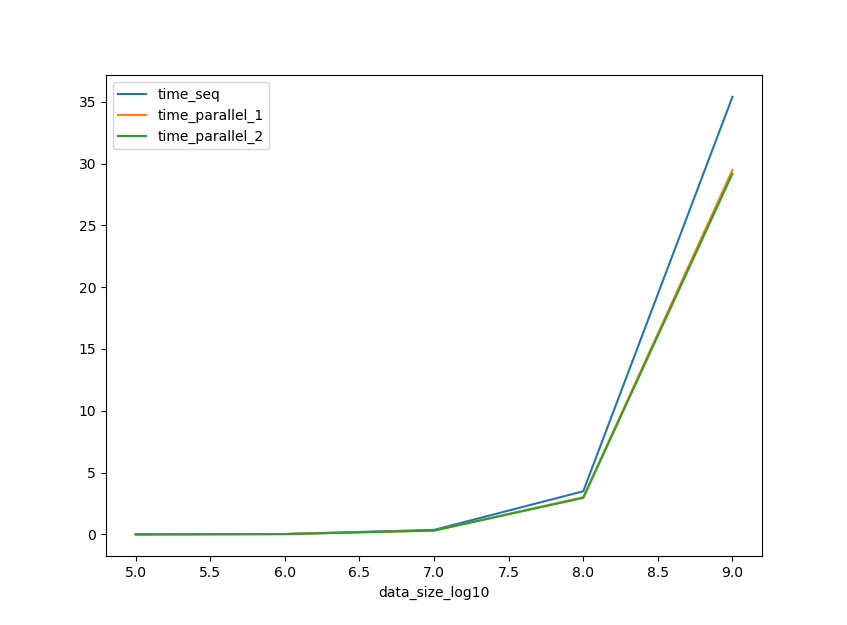
\includegraphics[width=0.8\linewidth]{assets/time_graph.png}
    \caption{Analysis of Time consumed by thread(s) for calculation of number of inputs (x-axis scaled to the log base 10)}
\end{figure}

\begin{figure}[H]
    \centering
    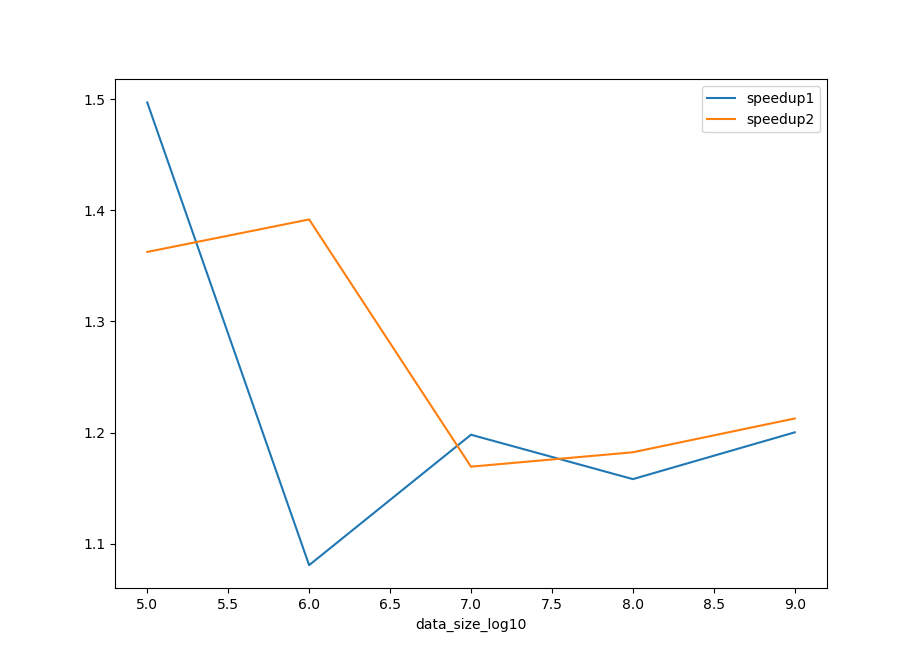
\includegraphics[width=\linewidth]{assets/speedup_graph.png}
    \caption{Comparison of speed up achieved from two method of parallelism}
\end{figure}

\section{Conclusion}
To get the speedup accurately the data and graphs values are based on summation of 100 iterations and it's been observed that for very initial where input vector size is about $ 10^7 $ then observed amount of time with parallel implementation is affecting negligible enhancement, however as the input size increase afterwards overall speedup observed about $ 1.21 $.


\end{document}

